 \documentclass{article}[10pt]% For LaTeX2e
\usepackage{nips15submit_09}

\usepackage[backend=bibtex]{biblatex}

\addbibresource{ref.bib}


\usepackage{amssymb}
\usepackage{newclude}
\usepackage[normalem]{ulem}
\usepackage{dsfont}

\usepackage{hyperref}
\usepackage{url}
\usepackage{amsmath}
\usepackage{graphicx}
% \usepackage{subcaption}
\usepackage{subfigure}
% \documentstyle[nips14submit_09,times,art10]{article} % For LaTeX 2.09

\usepackage{amsfonts}
\usepackage{amsmath}
\usepackage{amssymb}

\usepackage[]{algorithm}
\usepackage{algorithmic}
% \usepackage[noend]{algpseudocode} 

\newcommand{\R}{\mathbb{R}}

\title{Stochastic Neural Networks for \\Hierarchical Reinforcement Learning}


\author{
	Carlos Florensa, Yan Duan, Pieter Abbeel
}

% The \author macro works with any number of authors. There are two commands
% used to separate the names and addresses of multiple authors: \And and \AND.
%
% Using \And between authors leaves it to \LaTeX{} to determine where to break
% the lines. Using \AND forces a linebreak at that point. So, if \LaTeX{}
% puts 3 of 4 authors names on the first line, and the last on the second
% line, try using \AND instead of \And before the third author name.

\newcommand{\fix}{\marginpar{FIX}}
\newcommand{\new}{\marginpar{NEW}}

\nipsfinalcopy % Uncomment for camera-ready version

\begin{document}
	
	
	\maketitle

\begin{abstract}

Many practical problems in Reinforcement Learning (RL) only have a high level reward signal. This includes all tasks where a reward is only received when reaching a certain goal, even if many coordinated actions need to be taken before. Therefore these tasks have a \textit{sparse reward} and are considered some of the hardest in the field. To tackle them the two main approaches are reward shaping (eg. with some intrinsic motivation for exploration bonus) or using hand-engineered sequences of actions that allow to hierarchize the task and take high level actions (\textit{skills}, \textit{macro-actions} or \textit{options}). The first method can be completely unsupervised but the learning for one specific goal is difficult to re-use for another goal, even if the underlying dynamics are the same. The second method grants better re-use of skills but the prior knowledge needed to design the \textit{macro-actions} is undesired. In the present work we combine the best of both worlds to obtain \textit{skills} in a completely unsupervised fashion via a pre-training step and then use them to solve the actual task. We prove that a good "span of skills" can be learned using Stochastic Neural Networks (SNN) given their extra expressive power. The property of yielding different solutions to the MDP at the end of training (instead of a single one as most RL algorithms) is very interesting and we outline other uses in domain adaptation and bad local minima avoidance.
\end{abstract}

\section{Introduction}

% - What is the problem?
% - Why is it interesting and important?
% - Why is it hard? (E.g., why do naive approaches fail?) OK
% - Why hasn't it been solved before? (Or, what's wrong with previous proposed solutions? How does mine differ?)
% - What are the key components of my approach and results? Also include any specific limitations.


Recent advances in Deep Reinforcement Learning allow to train agents with super-human performance in tasks with discrete action-space like Go \cite{2016go} or some Atari games \cite{mnih2015human}. Nevertheless, many challenges remain in the continuous state-action environments, and in particular the problem of tasks with sparse reward is even more acute in the continuous case. In robotics, tasks like navigation or manipulation only have a natural reward in the goal position, and it is often hard to provide constant supervision along the trajectories with a cost function tailored to the task [cite IRL litterature?]. The main difficulty is that a sequence of well coordinated actions, producing a purposeful motion, is required to get any reward signal. Hence, as has been reported in the recent benchmark for continuous control tasks \cite{yuan2015}, it is very unlikely that the usual $\epsilon$-Greedy or Boltzmann exploration [ref] or adding Gaussian noise to the controls for policy gradient algorithms [TRPO], will yield a trajectory providing any feedback. 

To tackle this issue/challenge there are two main approaches and in this paper we will combine the best of both. One consists in providing an exploration bonus to the agent so that, despite not getting to the goal, it is still pushed to explore unseen regions that could potentially contain the extrinsic reward. In discrete MDPs this intrinsic reward may take many forms, from the simplest based on state-counting (rewarding each state inversely proportional to a function of its visitation counts) [refm, DM, simHash] to information theory-based like surprisal [ ref!! ]. In the continuous domain, VIME uses variatinal inference in Bayesian neural networks to incentivize exploration.

it is common to provide a specific abstraction of the problem.

\section{Methodology}

\subsection{Preliminaries}
\begin{itemize}
    \item describe MDP?
    \item introduce learning agent-centric skills
    \item introduce "intrinsic rewards" (COM speed)
    \item 
\end{itemize}

Words from ICLR call for papers:
- Unsupervised
- Representation learning for planning and reinforcement learning
- Hierarchical models
- application to robotics

% \section{Introduction}
% Most approaches to solve Reinforcement Problem yield a single policy at the end of the training procedure. And when this policy is stochastic, it is usually a parametrized unimodal Gaussian or discrete distribution. This limitation in the expressiveness of the policy has several drawback in terms of transfer of the final policy to modified MDPs, .

% First, it makes the final policy less robuts to changes in the MDP at test time, like in a transfer from simulation to reality setting, a model mismatch or simply when we try to generalize beyond the specific states it saw during training. 


% Feedforward Stochastic Neural Nets (FSNN) seem to be a natural way of representing multi-modal distribution functions \cite{Tang2014_FSNN}. We will show that in Reinforcement Leraning (RL), having such additional expressive power on the policy is beneficial, mainly during training. First, if different paths are equally rewarded, a more expressive policy will not suffer from ``competing updates", where different rollouts suggest to modify the policy in opposing ways, hence possibly cancelling the updates and slowing the learning. We provide examples where using latent variables in the Neural Network representing the policy improves learning compared to using regular unimodal Gaussian policies. It is shown that multimodal policies are learned, hence being able to accommodate conflicting learning experiences in a more efficient way. Secondly, this ability of maintaining several modes, each being a ``good" behavior for a the considered MDP, is of high interest in RL. In the context of transfer learning or going from simulation to reality, it is valuable to have a ``library" of possible strategies as some of the learned ones will not transfer properly. Furthermore, this span of skills can later be used as primites to solve more complex tasks in a hierarchical way. Finally, it could be argued that the learning process will be less prone to converging too early and getting stuck in a local minimum because the exploration will not be narrowed down so early thanks to the latent variables. 

% #######


% Recently it has been demonstrated that agents trained with Reinforcement Learning (RL) can surpass human experts in many discrete domains like Atari \cite{mnih2015human} or Go \cite{2016go}, but many challenges remain in the continuous case. To tackle locomotion or navigation problem under this framework that only has access to "trial-and-error", the most widely used methods are Policy Gradient. These methods behave better with the dimensionality of the action-state spaces than discretization approaches but they suffer from high variance. In most cases convergence to a local optima can be proven but in environments with high symmetry or similar rewards for different rollouts the learning can be quite slow. This is due to the limited expressive power of the family of probability distributions from where we select the policy. In this paper we propose to use extra latent variables in the Neural Network, hence having a much more extend family of probability distributions. We demonstrate a considerable speedup in highly symmetric MDPs when adding few latent variables. If more expressive power is desired and extra latent variables are added, a detriment in the learning speed is observed. We hence introduce a re-sampling method that, without extra interactions with the environment, is able to restore the performance improvement.

% The rest of the paper is organized as follows. In Section \ref{sec:reinforcement} we introduce in more depth Reinforcement Learning and Policy Gradient method, along with the common practices as for policy selection. In Section 3 we expose an intuitive argument explaining the additional expressive power obtained when adding latent variables to the Neural Network. In section 4 we describe how using this new family of probability distributions modifies the Policy Gradient algorithms. In Section 5 we introduce the "hallucination" resampling trick to deal with large number of added latent variables. Results of all these methods are presented in Section 6 and we finalize by discussing some promising future work directions.

% \section{Background material (this will be shrinked/skipped)}
% \subsection{Markov Decision Processes}
% The problems we wish to solve using RL are typically framed as follows: in discrete time, $t$, an agent exists in a state, $s_t$, chooses an action, $a_t$, and as a result transitions into a subsequent state $s_{t+1}$, according to an unknown transition probability $P(s_{t+1}|a_t,s_t)$.  It may then receive a reward signal $r_t$, from the environment for having made said transition, and the agent continues as permitted until the end of an episode.  The reward placement is also part of the environment and hence unknown to the agent, and must be explored by experience.  Usually the environments considered are time-independent and Markovian, meaning the next state's dependence on previous states an actions extends only to the immediately previous step.

% \subsection{Policy Representation}
% A common approach to the agent's decision-making in this problem is use a function, $\pi=\pi(a|s)$, which has as input the current state and returns an action to take.  The policy function is usually represented in terms of some (large) set of parameters, $\theta$, which for our purposes are the weights of a neural network (NN).  Several aspects of the learning method are made possible by using a probabilistic policy---the NN outputs values used to parameterize a random distribution which is then sampled to choose the action. The most common setting is to interpret the NN output values as the mean and variance of a multivariate Gaussian distribution.


% The overall goal of the agent is to learn behavior, meaning learn values of $\theta$, to maximize the expected returns, $R$, of trajectories, defined as,
% \begin{equation}
% \eta(\theta) = \mathbb{E}_\tau \left[R(\tau)  \right] = \mathbb{E}_{p(s_t,a_t)\sim \pi_\theta} \left[ \sum_{t=0}^T \gamma ^t r(t)  \right] = \int P_\theta(\tau)R(\tau)d\tau
% \end{equation}

% The coefficient $\gamma$ is a discount factor (e.g. $0.99$) used to promote gaining rewards earlier rather than later, and $\tau$ represents an entire trajectory ($s_0,a_0,s_1,a_1,...s_T$), which has a probability $P_\theta(\tau)$ and a total reward $R(\tau)$ associated with it.  The rightmost expectation is taken over all state-action sequences according to their likelihood in the environment under the policy $\pi_\theta$ (remember the policy is probabilistic, and the environment may or may not be).  This expectation value can be estimated by repeatedly playing out a policy in the environment from the given starting state and recording the rewards earned.  This is known as collecting ``rollouts''.

% \subsection{The Policy Gradient}
% Simply testing every possible policy is infeasible due to the curse of dimensionality.  Instead, it is preferable to gain from experience not only an estimate of the value of $\eta(\theta)$, but also an estimate of how to change theta to improve $\eta$, namely, the gradient $\nabla_\theta \eta$.  The gradient estimate can be obtained on an episodic basis with the likelihood trick, not derived here:
% \begin{equation} \label{eq:vanilla_grad}
% \nabla_\theta \eta = \mathbb{E}_{p(s_t,a_t)\sim \pi_\theta} \left[ \left( \sum_{t=0}^T \nabla_\theta \log{\pi_\theta(a_t|s_t)} \right) \left( \sum_{t=0}^T \gamma ^t r(t) \right) \right] 
% \end{equation}
% This provides a more efficient mean of searching the space of possible functions: gather experience, estimate the gradient of the expected return (using the recorded rewards and by backpropagation through the NN over all state-action samples collected), increment the policy parameters in that direction, and repeat to convergence.

% \par The empirical estimate of the expectation above suffers of high variance. Usually many tricks are applied to reduce it, like considering only future rewards or subtracting to them a baseline consisting of the approximate value function  \cite{peters2008reinforcement}. Also other enhancements, known as Natural Gradient Methods, can take into account the local curvature of the functional manifold parametrized by $\theta$, using the Fisher information matrix \cite{pascanu2013revisiting}. Finally an additional backtracking line search can be performed while estimating $\eta$ at the future point and shrinking the step if necessary. This last method is known as Trust Region Policy Optimization \cite{schulman2015trust} and is the one used in all our experiments. No further details are give as the only modification that will be needed to accomodate more expressive probability distributions as policies will be in the gradient estimate in \ref{eq:vanilla_grad}. In the next section we introduce why adding latent variables to the input of the NN parametrizing the policy can grant this extra expressive power.

% \section{Methodology}
% Our method for efficiently learning a span of skills is based on Stochastic Neural Networks. In Section \ref{sec:SNNs} we define them and understand their additional expressive power. Then in \ref{sec:PGwithSNN} we present the needed modifications to train them using Policy Gradient methods like TRPO \cite{schulman2015trust}. Finally in Sec.\ \ref{sec:Selector} we describe the architecture to re-use the learned span of skills in sparse reward tasks.

% \subsection{Stochastic Neural Networks}
% \label{sec:SNNs}

% \subsubsection{Definition and implementations}


% \subsubsection{Implementation: append noise to the observations}
% The most straight forward way of applying non-linearities to the \textit{latent} variables is simply appending noise as additional inputs to the NN. Whenever an action is taken, a value of a fixed probability distribution is sampled and together with the current observation (in the point MDP case, always 0), they determine the mean and variance of a Gaussian from where we finally sample the action. Notice that the parameters of the \textit{latent} variables are not part of the optimization and they do not depend on the current observation. The tested distributions for the latent variables will be a Normal Gaussiand or a Bernoulli.  

% \subsubsection{Additional expressive power}
% As explained in the previous section, the most standard use of Neural Nets to approximate probability distributions conditioned on some input $s$ , like a policy $\pi (a|x)$, is to deterministically process the input and then interpret the output of the NN as the mean and variance of a multivariate Gaussian distribution. This can be restrictive and indeed it can be seen as only allowing a simple affine transformation of some initial randomness $\epsilon \sim \mathcal{N}(0,1)$ as:
% $$
% a\sim \pi_\theta(a|x) = \mathcal{N}(\mu_\theta, \sigma_\theta) = \mu_\theta + \sigma_\theta \epsilon
% $$
% If we ask for more expressive power of this probability distribution, we could have the neural network output the parameters of a multimodal gaussian $(\mu_{\theta_i},\sigma_{theta_i})$ and the mixture weights $m_i$. Then this could be interpreted, for example, as also sampling from a uniform distribution $\upsilon \sim \mathcal{U}([0,1])$ and then picking the mixture that correspond to the interval where $\upsilon$ fell:
% $$
% a\sim \pi_\theta(a|x) = \sum_{i=1}^M m_i \mathcal{N}(\mu_{\theta_i}, \sigma_{\theta_i}) = \sum_{i=1}^M \huge\mathds{1}_{\sum_{j=1}^{i-1} m_j \leq \upsilon < \sum_{j=1}^{i} m_j} [\mu_{\theta} + \sigma_\theta \epsilon]
% $$
% Therefore, we see that the change is basically applying non-linearities to the randomness, here both in the indicator function (that could be avoided with other formulations) and the product of the two functions (which is necessary). To reach the next level of generality we would like to apply more tunable non-linearities to the randomness, for example passing it through a NN! Now there are many ways of doing so, with more or less structure and different trainabilities. For example a FSNN \cite{Tang2014_FSNN} includes some "stochastic units" that are simply binary variables sampled from a Bernouilli with a probability $p_{\theta}(x)$ that depends on the input $x$. This has a very clear interpretation of "switches" between modes.

% \subsection{Policy Gradient Methods with SNNs}
% \label{sec:PGwithSNN}
% In the following we will keep the discussion general and not consider the architecture details. Hence we will just refer to the output of the non-linearities applied to the initial random variables as the stochastic hidden or latent variable $h \sim P_\theta(h| s)$. The action is $a\sim \pi_\theta(a| s, h)$ and we will also refer to the probability of a certain path as $P_\theta(\tau, h)$where $\tau = (\vec s, \vec a)$. The naive formulation of including the hidden states in the objective will give:

% \[ \int P_\theta(\tau, \vec h) R(\tau) d \tau d h = \int \left( \int P_\theta(\tau, \vec h) dh\right) d \tau = \int P_\theta(\tau) R(\tau) d \tau \]

%  We arrive at the same objective as in the regular Reinforcement learning case. We can proceed to express the policy gradient as an expectation: %However, if we use the leftmost formulation and compute the policy gradient, we get the following 

% \begin{eqnarray*}
% 	&&\nabla_\theta \int P_\theta(\tau, h) R(\tau) d \tau d h \cr
% 	&=& \nabla_\theta \int P_{\theta_{old}}(\tau, h) \frac{P_{\theta}(\tau, h)}{P_{\theta_{old}}(\tau, h)} R(\tau) d \tau d h \cr
% 	&=& \nabla_\theta \int P_{\theta_{old}}(\tau, h) \frac{\pi_{\theta}(\vec a | \vec s, \vec h) P_\theta(\vec  h | \vec s)}{\pi_{\theta_{old}}(\vec a | \vec s, \vec h) P_{\theta_{old}}(\vec  h | \vec s)} R(\tau) d \tau d h \cr
% \end{eqnarray*}

% Evaluated at $\theta = \theta_{old}$, we get the following familiar policy gradient:

% \[ \mathbb{E}_{\tau, h \sim P_{\theta_{old}}(\cdot, \cdot)} \left[ \left(\nabla_\theta \log P_\theta(\vec a | \vec s, \vec h) + \nabla_\theta \log P_\theta(\vec h | \vec s) \right) R(\tau) \right]\]

% All this derivation almost did not distinguish between the probability of taking an action and the probability of sampling a certain latent variable. Nevertheless, in there is a fundamental difference that could be exploited for faster learning and we investigate in the next Section: notice that the actions cannot be "re-sampled" individually as the whole roll-out from that point on would have to change. But this is not the case for the latent variables $h$ as the action that was taken still has a certain probability of being taken even if the latent sampled latent variable is different! For a more in-depth study, see \cite{schulman2015gradient}.

% \subsection{Selector Network for hierarchical tasks}
% \label{sec:Selector}

% \section{Results}
% \label{sec:Results}
% \subsection{Point MDP with Bimodal Reward}
% First let's describe the basic MDP:
% \begin{itemize}
%     \item The time horizon is one single step.
%     \item The action is $a\in\R$ and the transition is $s'=a$
%     \item The reward is a deterministic bimodal "Gaussian" (see Fig.\ \ref{fig:basic_reward_function} ) $$R(s)=\frac{1}{\sigma\sqrt{2\pi}} \left(\frac{1}{2}e^{-\frac{(s-\mu_1)^2}{2\sigma^2}}+\frac{1}{2}e^{-\frac{(s-\mu_2)^2}{2\sigma^2}}\right)$$
% \end{itemize}
% The symmetry of this MDP makes it hard for gradient methods on unimodal policies, as can be seen in Fig.\ \ref{fig:basic_learning}, where there is a "flat" learning that can last up to 60 iterations. The evolution of the mean and var or the policy along the iterations can be seen in Fig.\ \ref{fig:basic_progress_policy}, where we observe a rapid decrease of the variance once the mean finally starts drifting towards one of the two modes.

% \begin{figure}[ht]
% \centering
% \subfigure[Deterministic reward function]{
%   \label{fig:basic_reward_function}
%   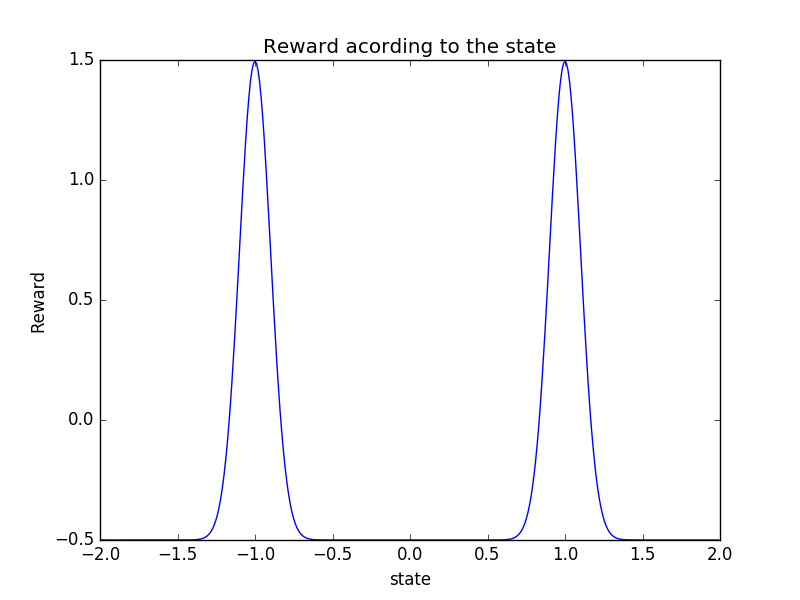
\includegraphics[width = 0.3\textwidth]{Figures/Reward_function_1Dbasic.png}
% }
% \subfigure[Learning curves for 3 random seeds]{
%   \centering
%   \label{fig:basic_learning}
%   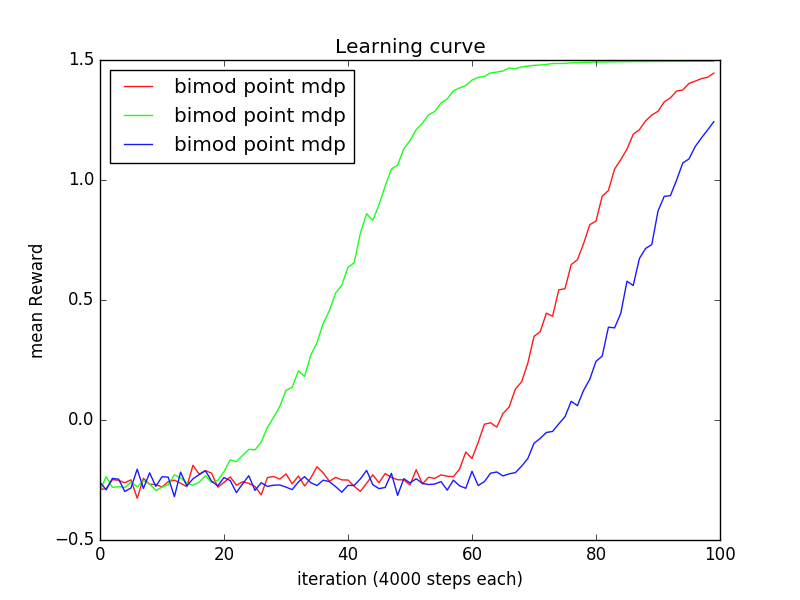
\includegraphics[width = 0.3\textwidth]{Figures/learning_curve_1Dbasic.png}
% }
% \subfigure[Evolution of mean and variance across iterations]{
%   \centering
%   \label{fig:basic_progress_policy}
%   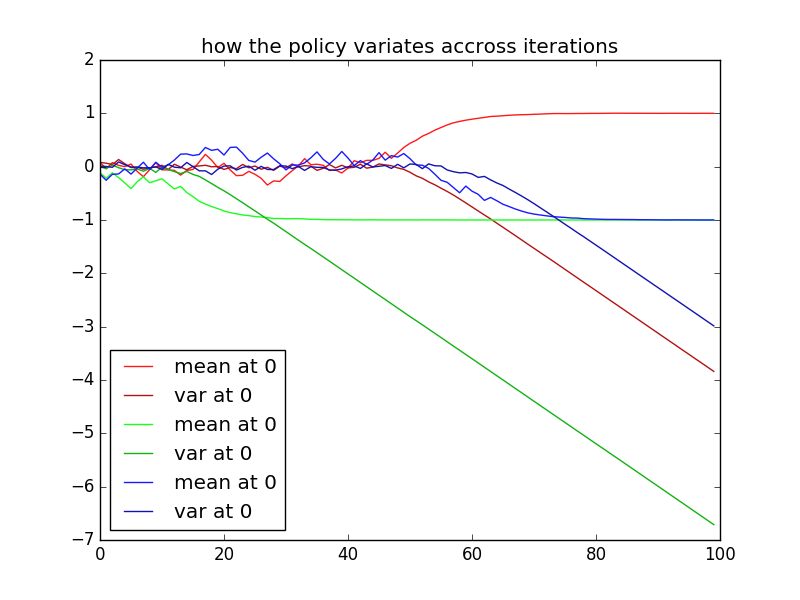
\includegraphics[width = 0.3\textwidth]{Figures/policy_progress_1Dbasic.png}
% }
% \caption{The point MDP with bimodal reward solved with TRPO with batches of 500 steps and using a uni-modal Gaussian parametrized by an (8,8) MLP}
% \label{fig:basic_bimodal}
% \end{figure}

% The strongest bimodality after training on this problem is observed when using 2 independent Gaussian random varaibles as latents, as seen in Fig.\ \ref{fig:snn_final_policyMC}. This is surprising as the randomness is continuous, and indeed we see that it has some difficulties \ref{fig:snn_learning_curve}, mainly due to not narrowing the variance around the 2 high reward points (1 and -1): it cannot learn such a steep step function.

% \begin{figure}[ht]
% \centering
% \subfigure[Learning curves for 3 random seeds]{
%   \centering
%   \label{fig:snn_learning_curve}
%   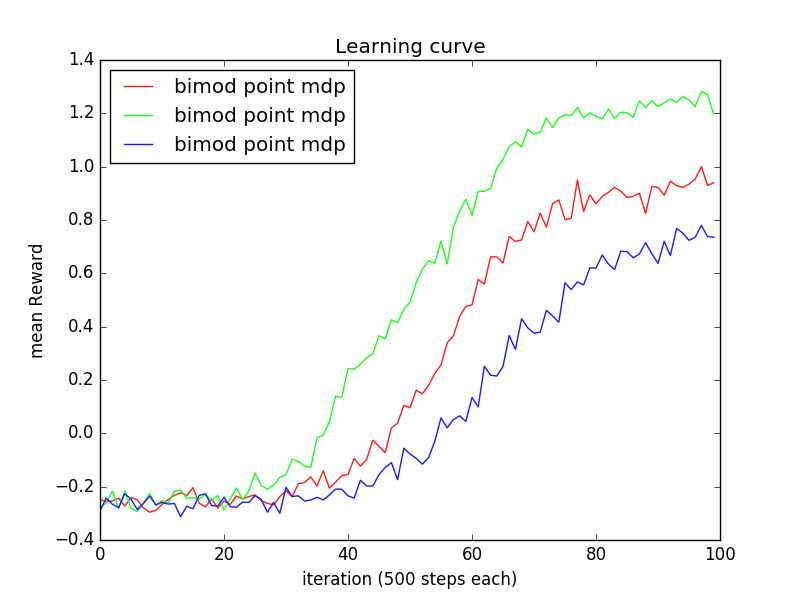
\includegraphics[width = 0.45\textwidth]{Figures/snn_1Dbimod_normal/learning_curve_snn_2latent_norm_npo_500batch.png}
% }
% \subfigure[Final policy learned (MC estimated)]{
%   \label{fig:snn_final_policyMC}
%   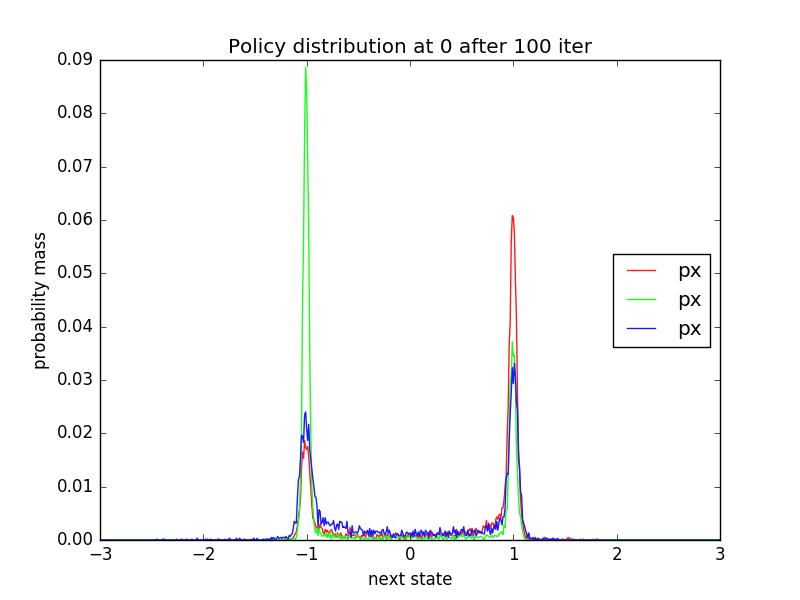
\includegraphics[width = 0.45\textwidth]{Figures/snn_1Dbimod_normal/MC_policy_learned_at0_iter100.png}
% }
% \caption{Performance of the SNN on first bimodal MDP, with 2 latent normal variables}
% \label{fig:snn_bimodal}
% \end{figure}

%  Much more interesting is what we observe when we use discrete distributions, as in Fig.\ \ref{snn_bimodal_discrete}. We observe that the learning time is reduced and the highest reward is achieved within the 100iterations in 2 of the 3 random seeds.
 
% \begin{figure}[ht]
% \centering
% \subfigure[Learning curves with 2 latent Bernouilli(0.5)]{
%   \centering
%   \label{fig:snn_learning_curve_bern}
%   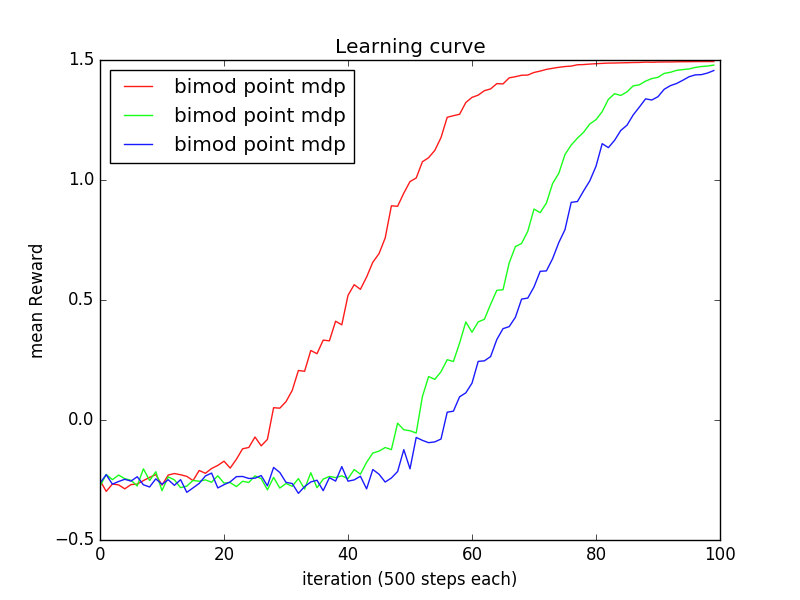
\includegraphics[width = 0.45\textwidth]{Figures/snn_1Dbimod_normal/learning_curve_bern.png}
% }
% \subfigure[Final policy learned (MC estimated) with 2 latent Bernouilli(0.5)]{
%   \label{fig:snn_final_policyMC_bern}
%   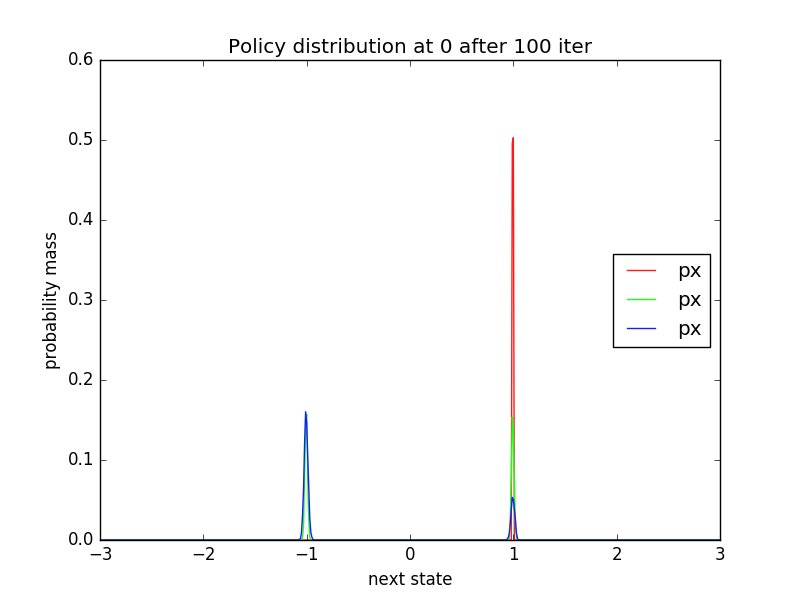
\includegraphics[width = 0.45\textwidth]{Figures/snn_1Dbimod_normal/MC_policy_learned_at0_bern.png}
% }
% \subfigure[Learning curves with 2 latent Binom(4,0.5)]{
%   \centering
%   \label{fig:snn_learning_curve_binom}
%   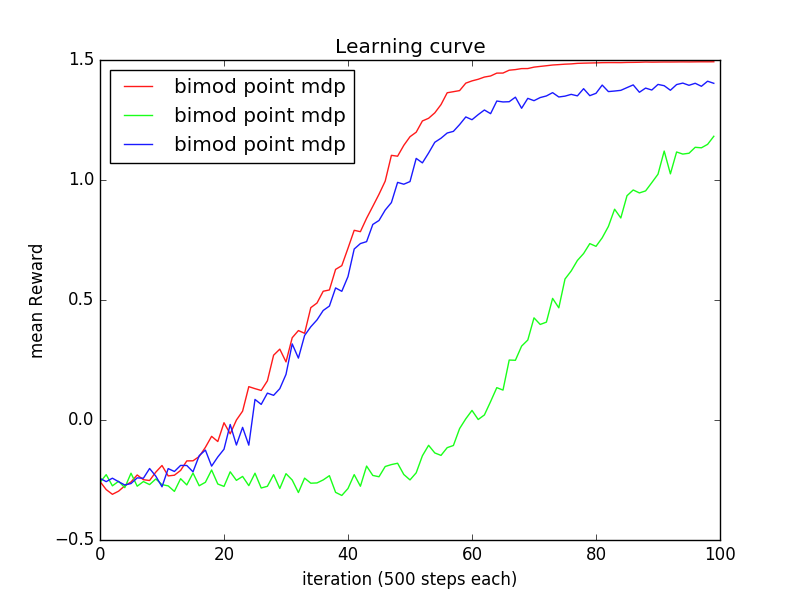
\includegraphics[width = 0.45\textwidth]{Figures/snn_1Dbimod_normal/learning_curve_2bino4.png}
% }
% \subfigure[Final policy learned (MC estimated) with 2 latent Binom(4,0.5)]{
%   \label{fig:snn_final_policyMC_binom}
%   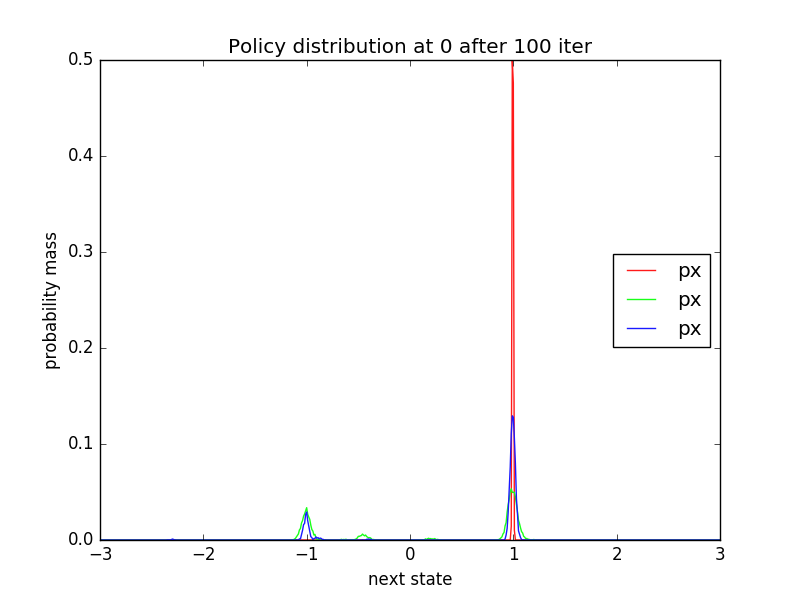
\includegraphics[width = 0.45\textwidth]{Figures/snn_1Dbimod_normal/MC_policy_learned_at0_2bino4.png}
% }
% \caption{Performance of the SNN on first bimodal MDP, with 2 latent discrete variables}
% \label{fig:snn_bimodal_discrete}
% \end{figure}

% \subsection{Swimmer in a Maze}


% \section{Discussion and future work}

% We have implemented and tried other ideas, like having a latent-variable dependent baseline. But at least in the cases we have tried it doesn't make that much of a difference, see Fig.\ \ref{fig:baselines}. We have also tried having stochastic units instead of inputs as described by the original paper on FSNN, but again no relevant effect has been observed in any of the MDPs we have considered.

% A ongoing work that will potentially help a lot int the continuous case is reducing the sampling of the latent variables to the first step of each rollout or to every so-many time steps. This will allow consistency of the mode during a full rollout, which might be the reson why adding latent variables to the continuous task hasn't seemed to improve them so far. It's like changing your mind constantly! So no value is accorded to the latents. Another even better way of doing this would be by having a recurrent neural net as a policy, that can hence remember what "line of actions" it was taking the previous time-steps.

% The most similar work we have found considers Energy-based policies like Restricted Boltzmann machines \cite{heess2012actor}. We will need to compare to them.

% \section{References}

% \printbibliography

% \appendix
% \section{Hallucination: resampling from the latents}

% In this section we introduce a resampling procedure that, without requiring new rollouts, can improve the estimate of the gradient. This is beneficial in the case of having expensive simulation or simply when dealing with real robots, much slower than simulation. The main idea is to enlarge the size of our batch size by duplicating the rollouts, and on each duplicated rollout the latent variables $h$ are re-sampled.

% \begin{algorithm}                     
% \caption{Hallucination step with $M$-resampling}          
% \label{alg1}                         
% \begin{algorithmic}                  
%     \STATE Collect $n$ full rollouts $\tau_i= (\vec s_i, \vec a_i, \vec h_i)$
%     \FOR{i = 1 \dots n}
%         \FOR{m = 1 \dots M}
%             \STATE Resample $\vec h^m_i \sim P_\theta(\vec s)$
%             \STATE Add to the rollouts set $\tau_i^m=(\vec s_i, \vec a_i, \vec h_i^m)$
%             \STATE Compute the importance weight $w_i^m=\exp(\log{\pi_\theta(\vec a_i| \vec h_i^m, \vec s_i)}- \log{\pi_\theta(\vec a_i| \vec h_i, \vec s_i)})$
%         \ENDFOR
%     \ENDFOR
%     \STATE Execute your favorite Gradient applying $w_i^m$.\\
% \end{algorithmic}
% \end{algorithm}

% \subsection{Hallucination allows more latents}
% In the simple MDP that we study in this examples the extra hallucinations do not further speedup the learning when a small number of latent variables is used. But it does become critical if too many latent variables are added as we can see in Fig.\ \ref{fig:effect_hallu}.

% \begin{figure}
% \centering
% 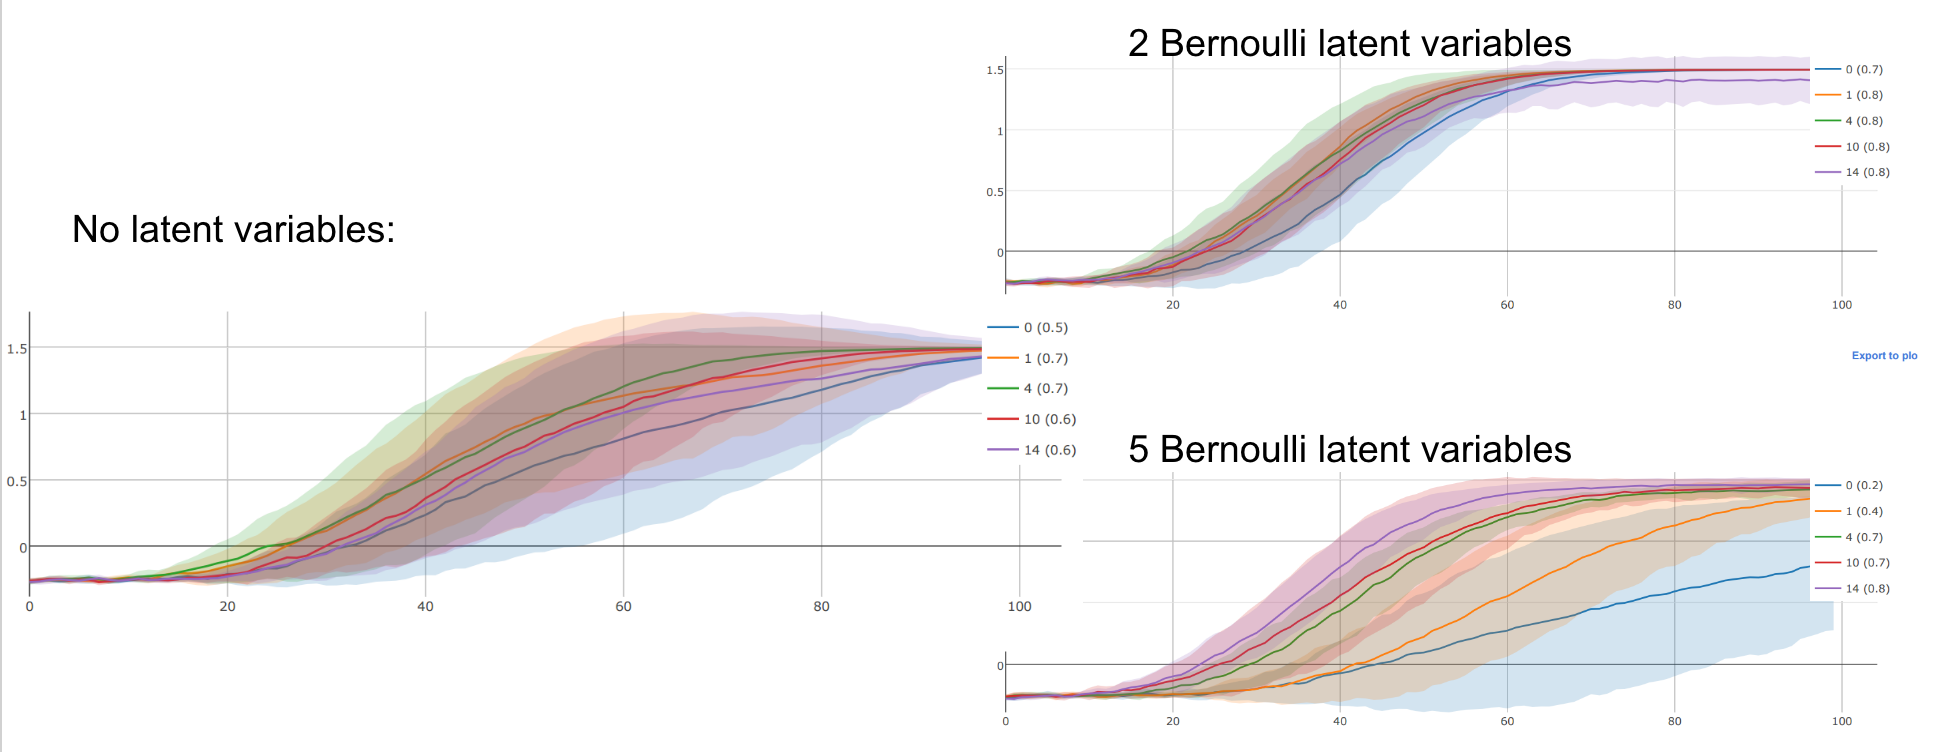
\includegraphics[width=\textwidth]{Figures/effect_hallu.png}
% \caption{Hallucination compensates the negative effect of adding more latent variables}
% \label{fig:effect_hallu}
% \end{figure}


\end{document}